\documentclass[11pt, fleqn]{article}

\documentclass[11pt, fleqn]{article}

\usepackage[usenames,dvipsnames,svgnames,table]{xcolor}
\usepackage{amsmath}
\usepackage{amsfonts}
\usepackage[margin=1in]{geometry} % To set the margin widths
\usepackage{graphicx}
\usepackage{listings}
\usepackage{multirow}
\usepackage{tabularx}
\usepackage{varioref}
\usepackage[noabbrev,capitalize]{cleveref}
\usepackage[group-separator={,}]{siunitx}
\usepackage{subcaption}
\usepackage{titlesec}
\usepackage{lscape}
\usepackage{bm}
\usepackage[titletoc,toc,title]{appendix}

\lstset{
  frame=single,
  basicstyle=\ttfamily,% print whole listing small
  language=R,
  aboveskip=3mm,
  belowskip=3mm,
  showstringspaces=false,
  columns=flexible,
  numbers=none,
  commentstyle=\color{ForestGreen},
  stringstyle=\color{Maroon},
  breaklines=true,
  breakatwhitespace=true,
  tabsize=2,
  literate={<-}{{$\gets$}}1 {~}{{$\sim$}}1
}

\sisetup{output-exponent-marker=\textsc{e}}

\setlength{\parskip}{12pt} % Sets a blank line in between paragraphs
\setlength\parindent{0pt} % Sets the indent for each paragraph to zero

% \crefname{figure}{Figure}{Figures}
% \crefname{section}{Section}{Sections}
% \crefname{table}{Table}{Tables}
% \crefname{lstlisting}{Listing}{Listings}

\setlength{\parskip}{12pt} % Sets a blank line in between paragraphs
\setlength\parindent{0pt} % Sets the indent for each paragraph to zero

\begin{document}

\title{Machine Learning (41204-01)\\HW \#2}
\author{Will Clark $\vert$ Matthew DeLio \\
\texttt{will.clark@chicagobooth.edu} $\vert$ \texttt{mdelio@chicagobooth.edu} \\
University of Chicago Booth School of Business}
\date{\today}
\maketitle

\section{kNN with 1 Attribute}

\begin{figure}[!htb]
  \centering
  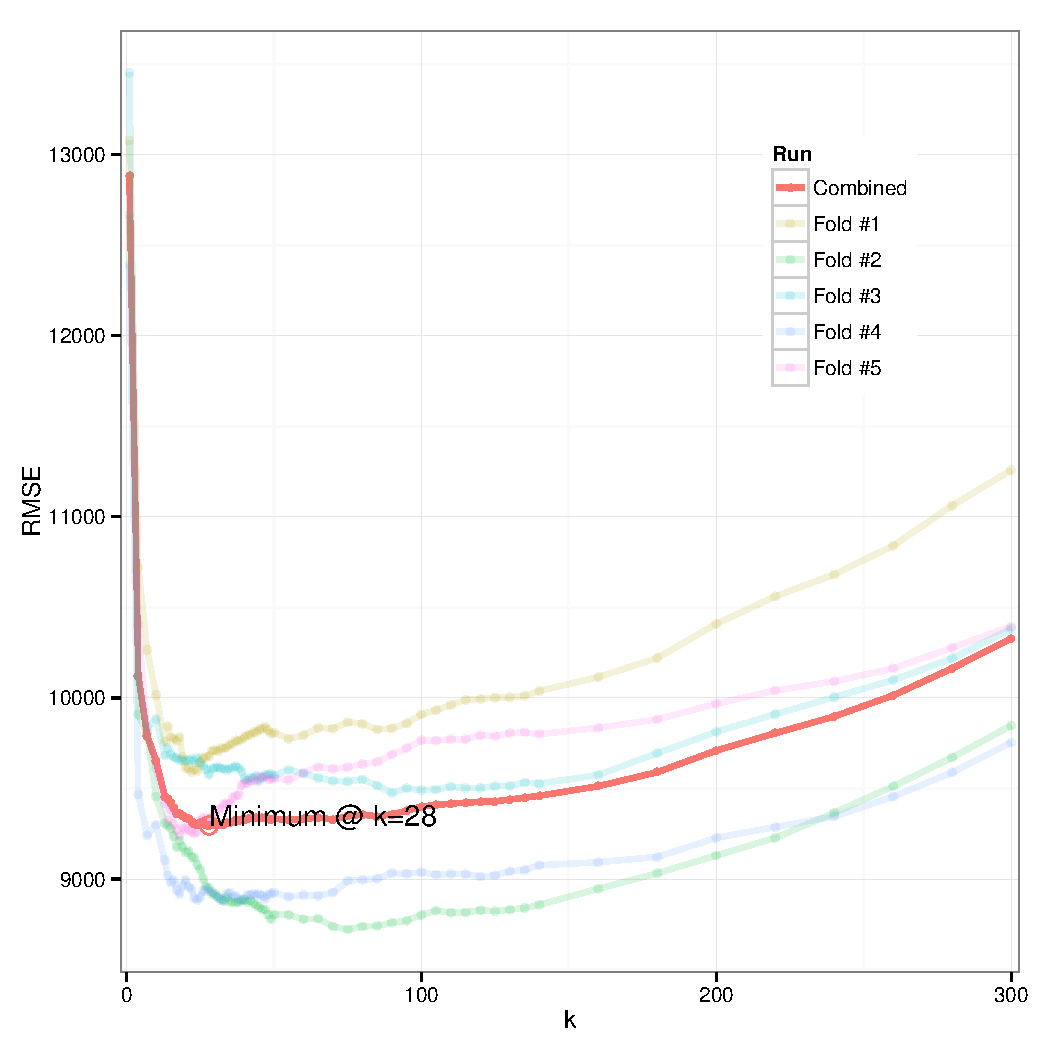
\includegraphics[scale=.5]{1p_cv_k.pdf}
  \caption{5-fold kNN CV for 1 Attribute}
  \label{fig:1p_k}
\end{figure}

\begin{figure}[!htb]
  \centering
  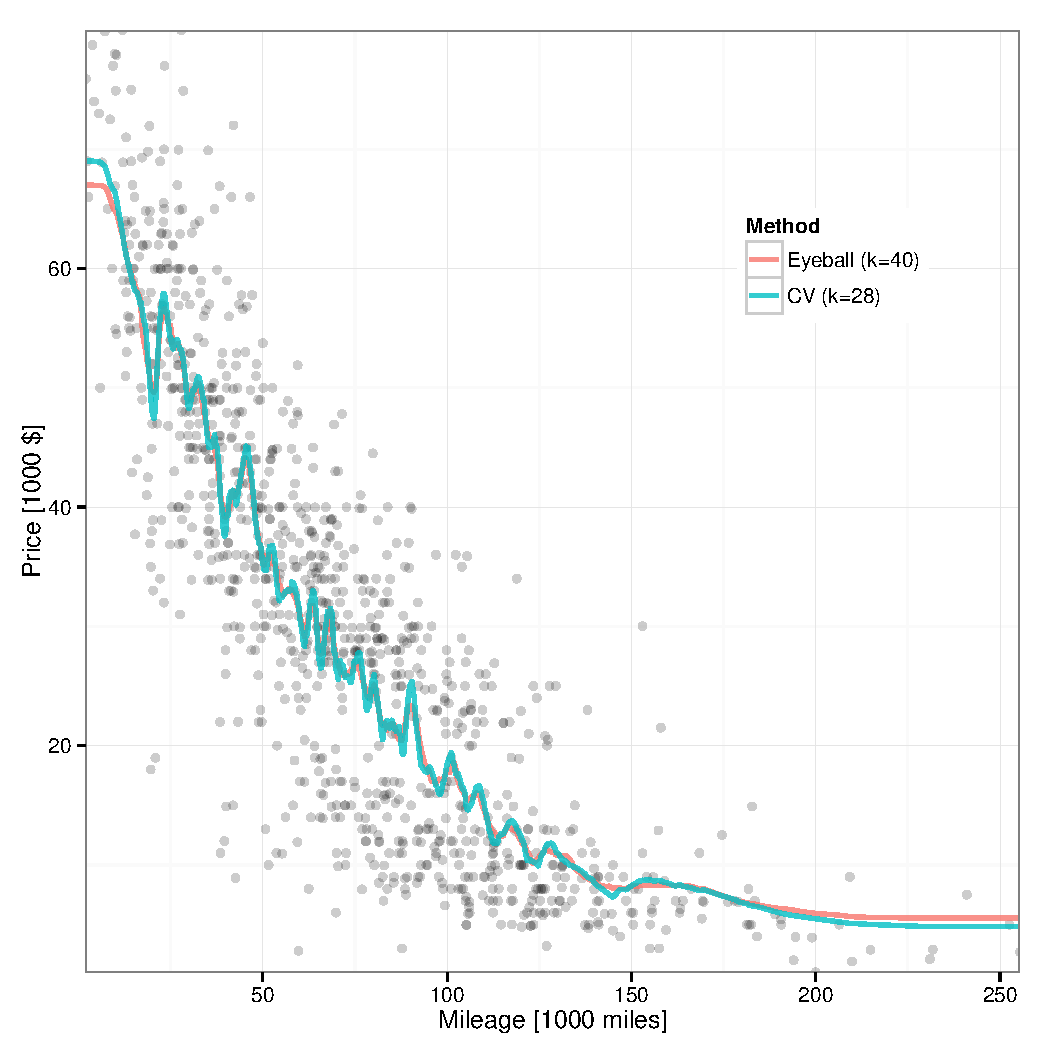
\includegraphics[scale=.5]{1p_fit_eye_ev.pdf}
  \caption{Comparison of Fit Between ``Eyeball'' and CV Chosen $k$'s}
  \label{fig:1p_fit}
\end{figure}

\subsection{Price Predictions}
% latex table generated in R 3.1.2 by xtable 1.7-4 package
% Sun Oct  4 21:25:06 2015
\begin{table}[ht]
\centering
\begin{tabular}{rrr}
  \hline
 & Mileage & $\hat(price)$ \\ 
  \hline
1 & 100000 & 16676.18 \\ 
   \hline
\end{tabular}
\caption{Predicted Value with 1 Attribute} 
\label{tab:1p_predict}
\end{table}


\section{kNN with 2 Attributes}

\begin{figure}[!htb]
  \centering
  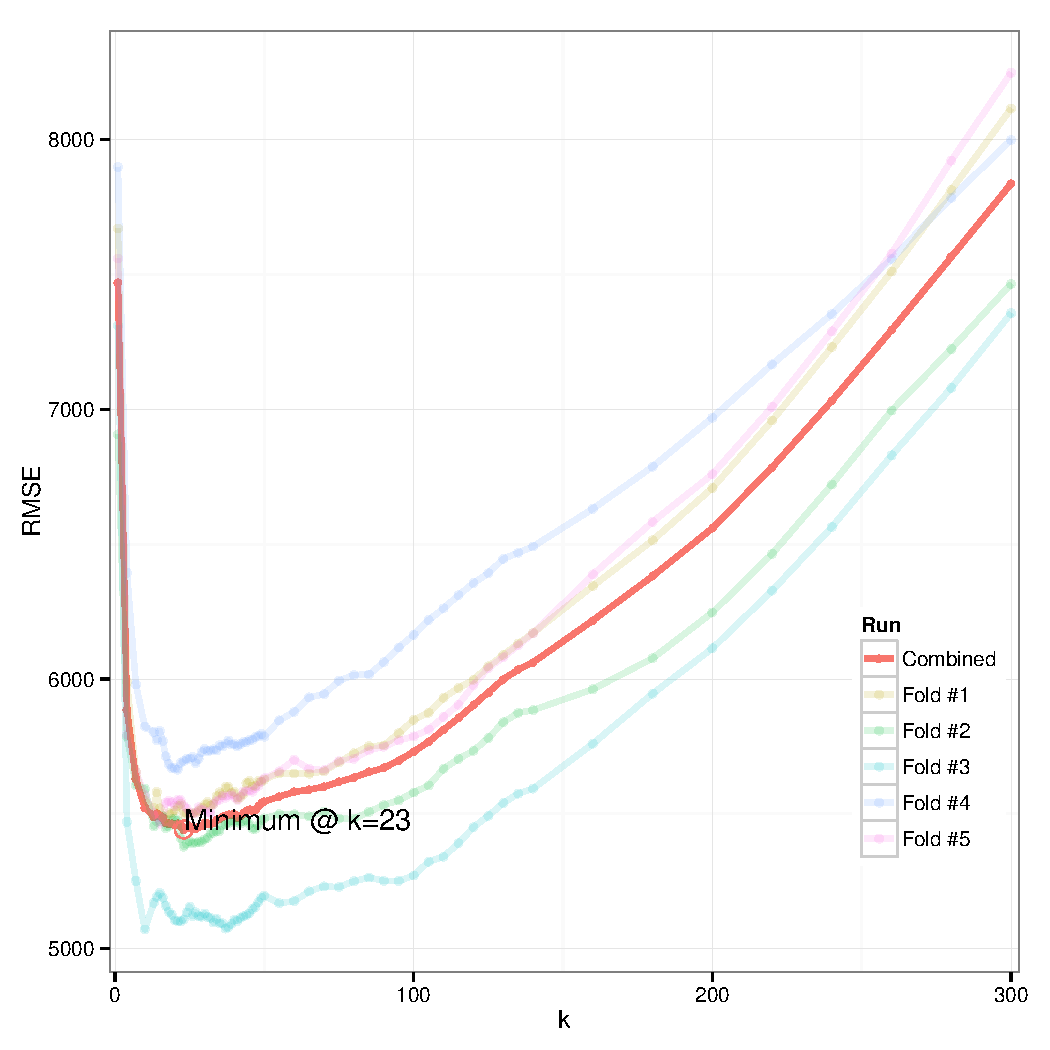
\includegraphics[scale=.5]{2p_cv_k.pdf}
  \caption{5-fold kNN CV for 2 Attributes}
  \label{fig:2p_k}
\end{figure}

\subsection{Price Predictions}
% latex table generated in R 3.2.2 by xtable 1.7-4 package
% Wed Oct  7 12:13:34 2015
\begin{table}[ht]
\centering
\begin{tabular}{rrrr}
  \hline
 & Year & Mileage & $\widehat{price}$ \\ 
  \hline
1 & 2008 & 75000 & 31678.22 \\ 
   \hline
\end{tabular}
\caption{Predicted Price with 2 Attributes} 
\label{tab:2p_predict}
\end{table}


\section{RMSE Comparison of kNN for 1 \& 2 Attributes}
\begin{figure}[!htb]
  \centering
  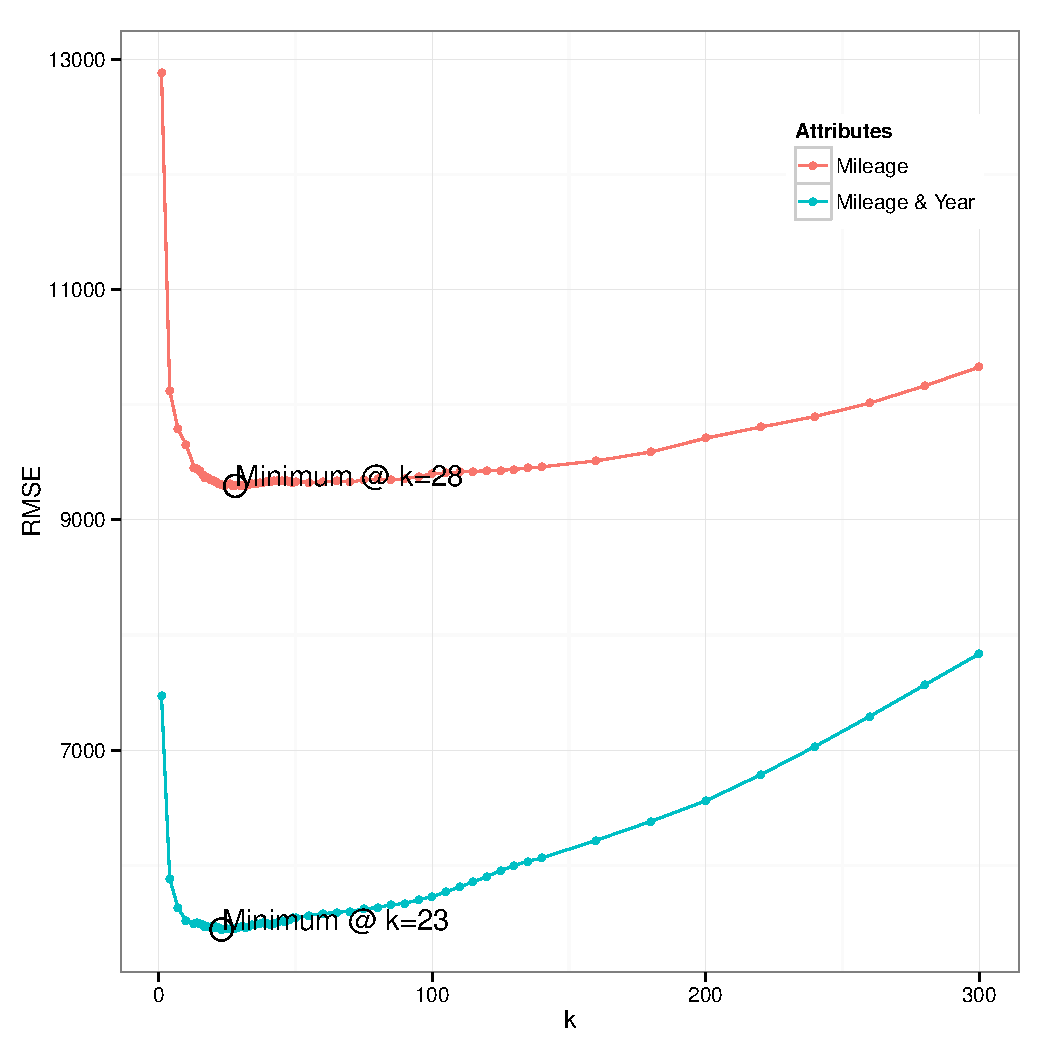
\includegraphics[scale=.5]{1p_2p_cv_compare.pdf}
  \caption{RMSE for 1 \& 2 Attributes}
  \label{fig:p_compare}
\end{figure}

\end{document}

% \input{.tex}

% \begin{figure}
%   \centering
%   \begin{subfigure}[b]{0.49\textwidth}
%     \includegraphics[width=\textwidth]{.pdf}
%     \caption{}
%     \label{fig:}
%   \end{subfigure}
%   \hfill
%   \begin{subfigure}[b]{0.49\textwidth}
%     \includegraphics[width=\textwidth]{.pdf}
%     \caption{}
%     \label{fig:}
%   \end{subfigure}
%   \caption{}
% \end{figure}

% \begin{figure}[!htb]
%   \centering
%   \includegraphics[scale=.5]{.pdf}
%   \caption{}
%   \label{fig:}
% \end{figure}

